\section{Charging Station Design}

Our design relies heavily on interfaces to allow testing the system through hardware simulations. It is thus easy to create a piece of code that sends the same signals to the system as the physical hardware inmplementation would, allowing for testing of the individual units before implementation. This is taken further, as the internal components of the system ( \textit{stationControl} and \textit{ChargeController}) interacts through an interface, allowing the \textit{chargeControlle} to be replaced for upgrades or testing of \textit{stationControl}.

The design of the charging station is displayed in \autoref{fig:class-diagram}. Central to the system is the \textit{stationControl} class, which handles all interaction with the user, through various interfaces (display, door and rfid detector). It also interacts with the \textit{chargeController} through another interface. The \textit{chargeController} meanwhile interfaces with the USB charger, cobntrolling it, and also displays charging status on the display through the display interface. 

\begin{figure}[h]
  \centering
  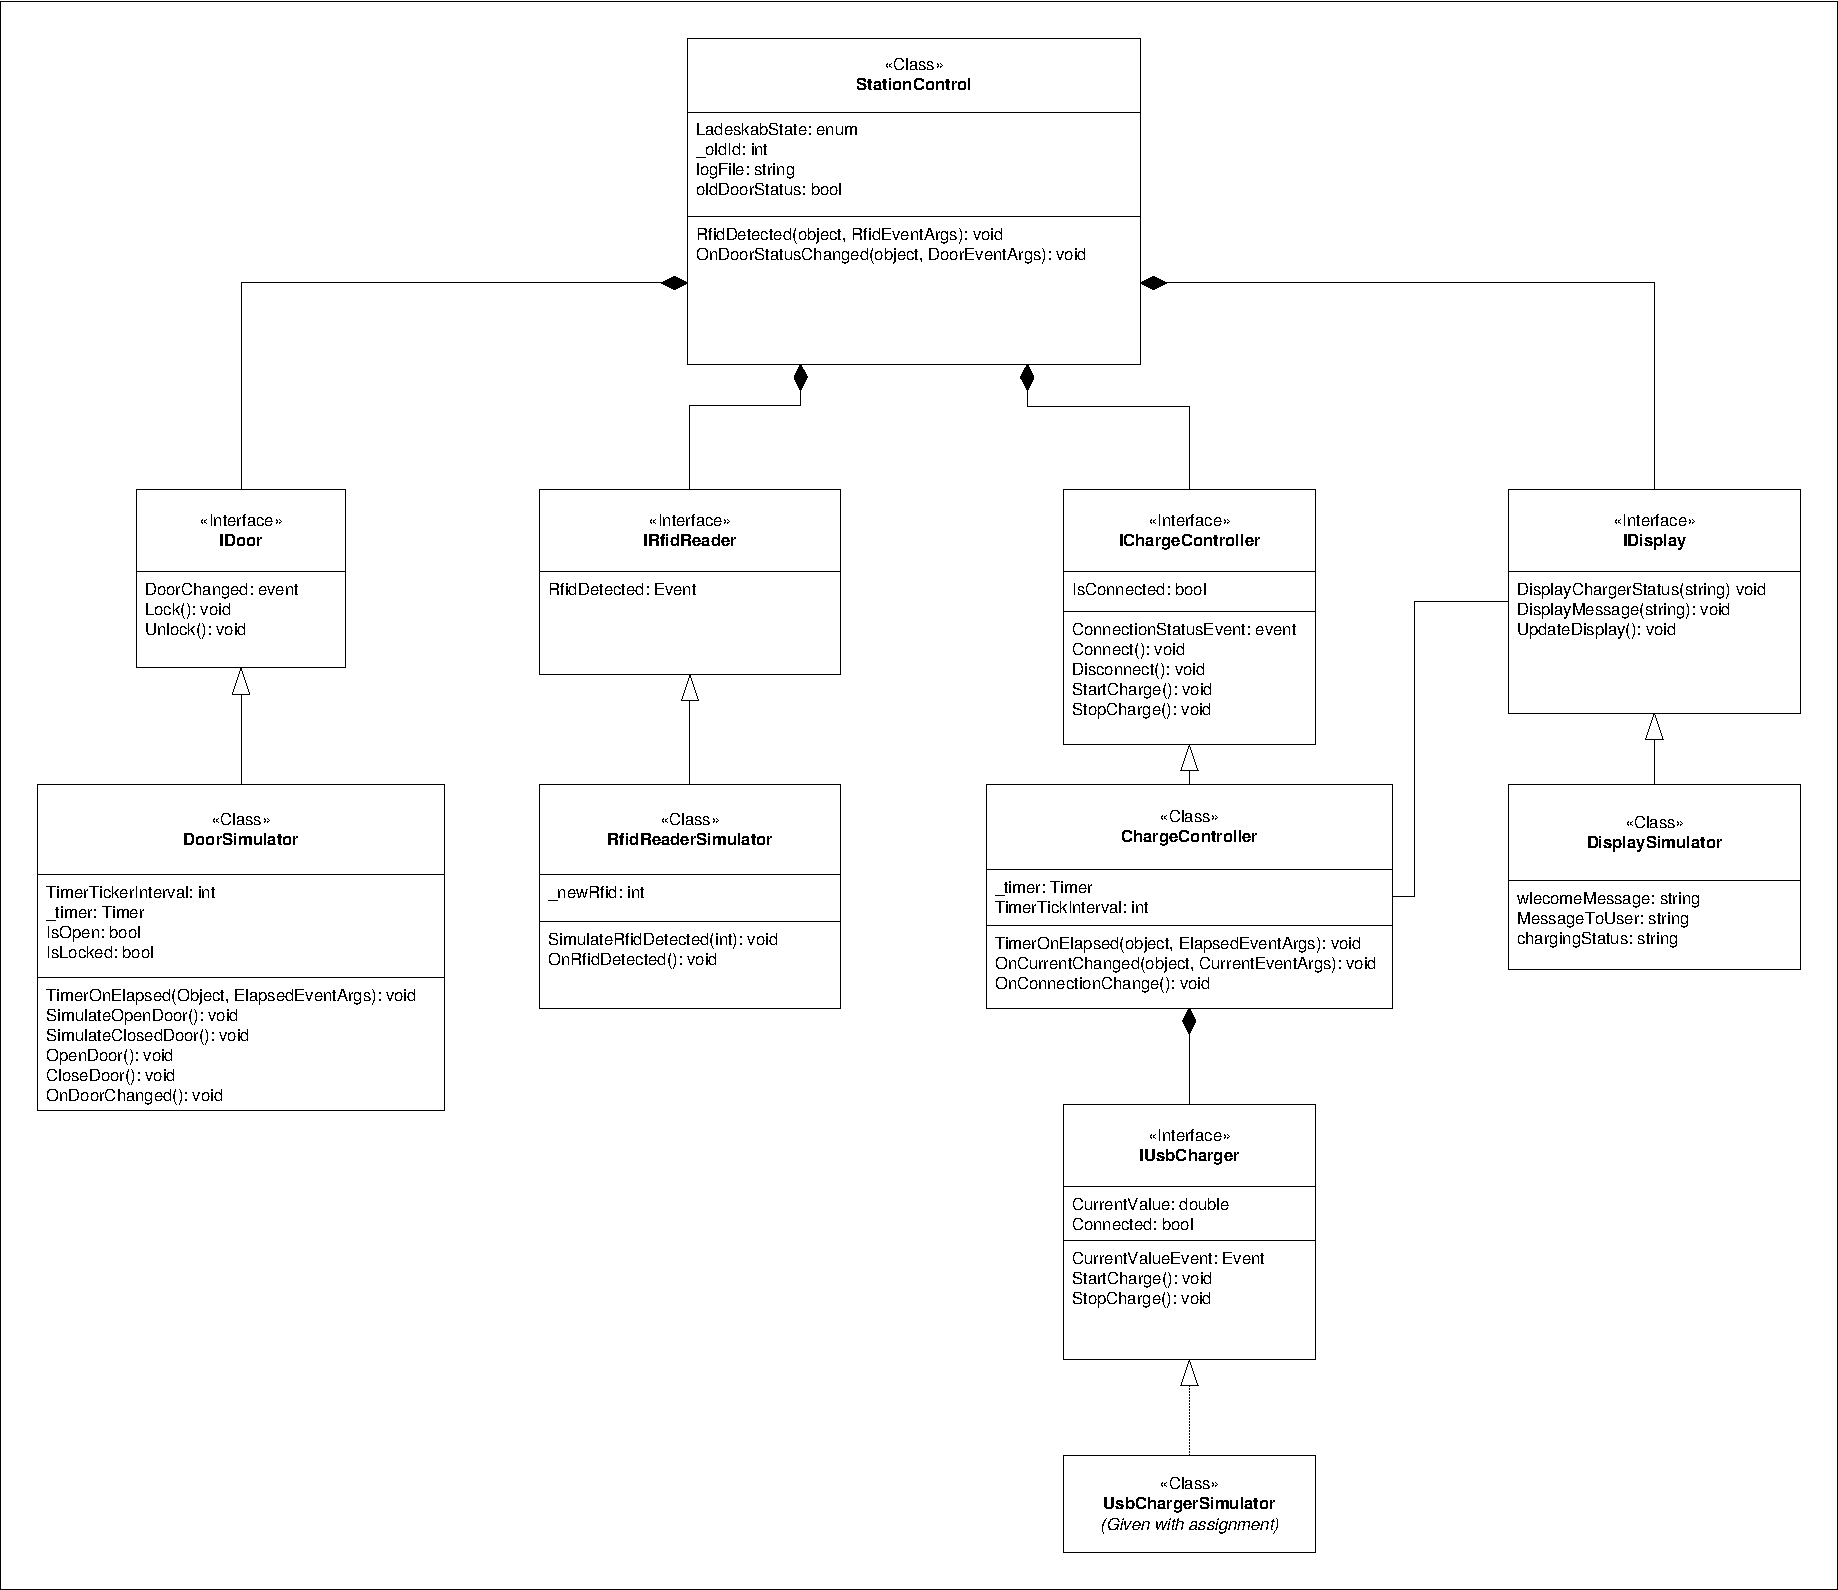
\includegraphics[width=\textwidth]{02-Body/images/ChargingStation_classDiagram.pdf}
  \caption{Class diagram for the charging station system}
  \label{fig:class-diagram}
\end{figure}

\vspace{3em}

The charging station is first activated by the door opening, causing the station to ask the user to connect the phone. The user then connects the phone and closes the door, which causes the station to ask for an RFID. If the phone has not been correctly connected (as cheked by the chargeController) the station reports this to the user through the display. If the phone has been properly connected when the RFID is detected the door locks and the station starts charging the phone. This continues until the charging is complete or the same RFID as was used to start the charging is detected. When the RFID of the user is detected after charging has begun, the system stops the charging and unlocks the door, alowing the user to disconect their phone.
This sequence is illustrated in \autoref{fig:seq-diagram}.

\begin{figure}[h]
  \centering
  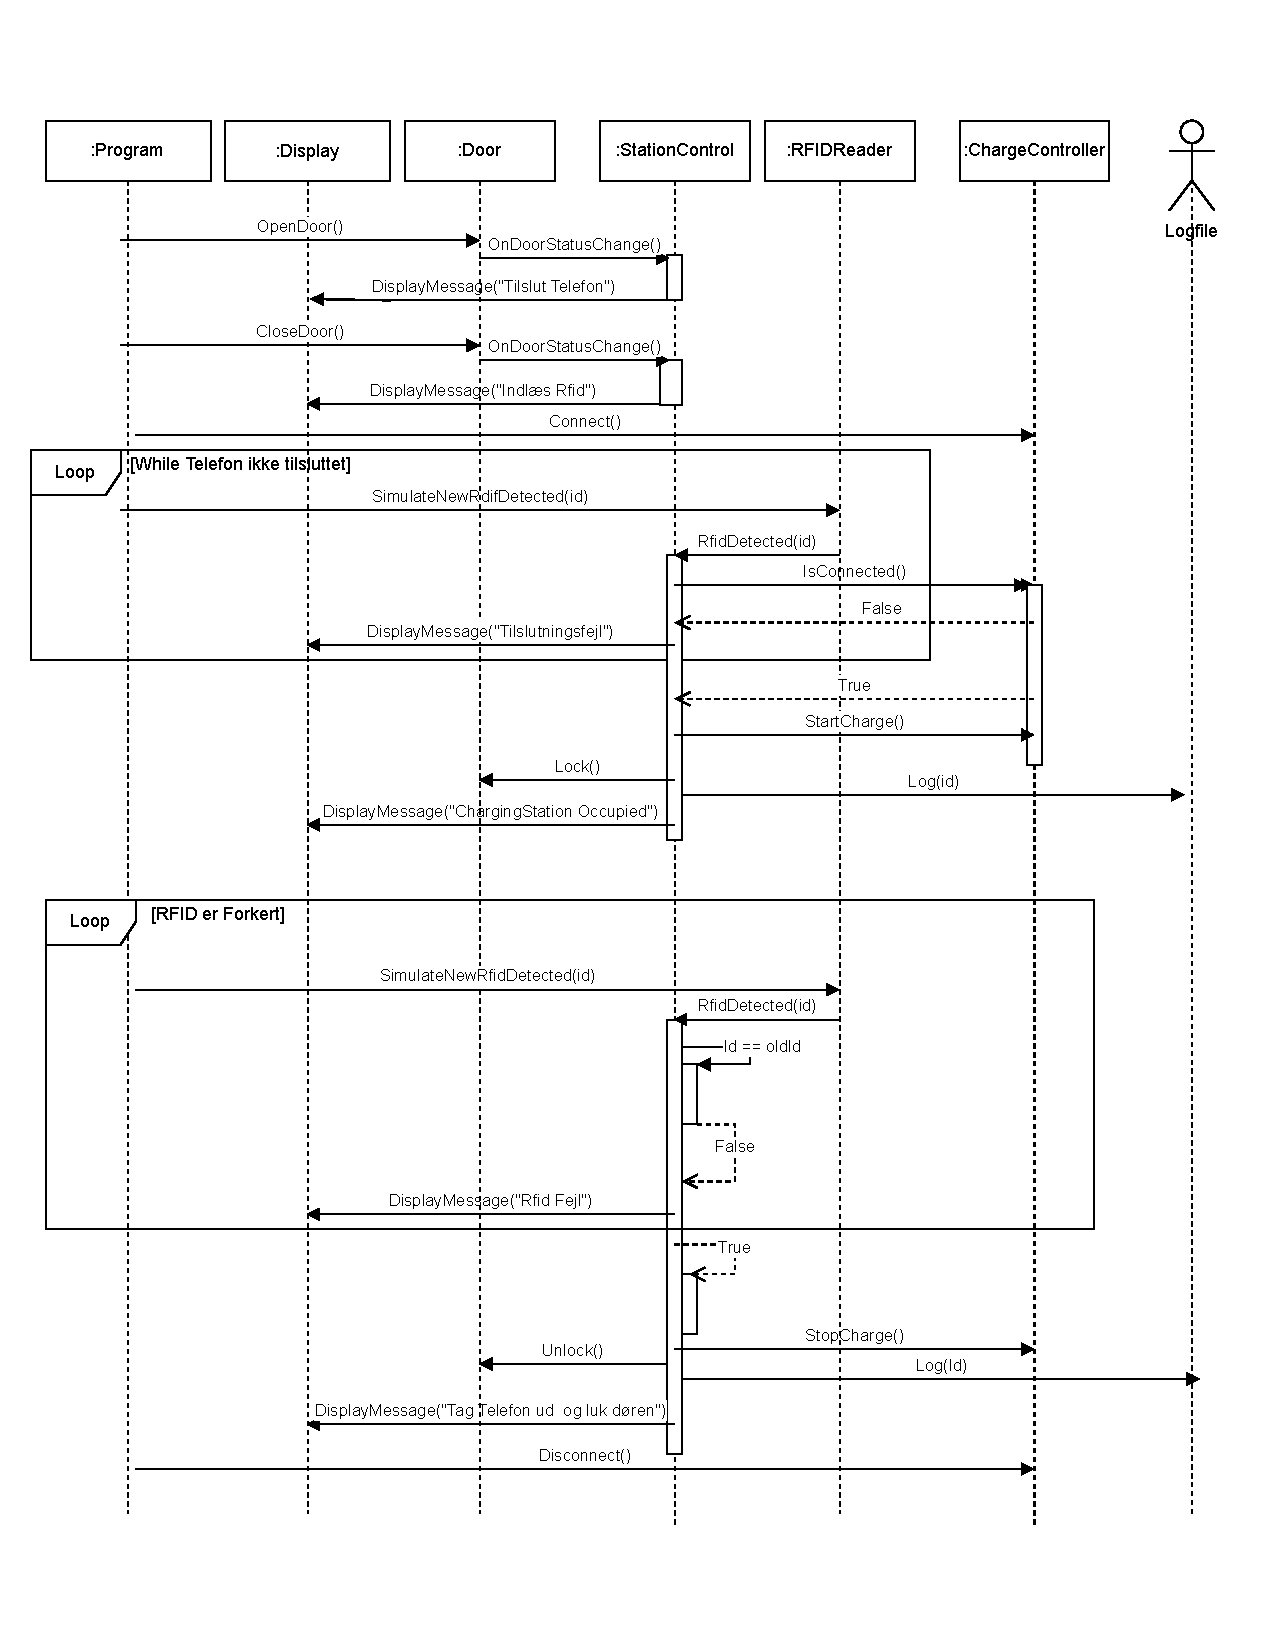
\includegraphics[width=\textwidth]{02-Body/images/SEQpdf.pdf}
  \caption{Sequence diagram describing normal opperation of the charging station}
  \label{fig:seq-diagram}
\end{figure}

